\documentclass[nobib]{tufte-handout}

\title{Föreläsning 2: Kombinatoriska bevis, binomialsatsen, kompositioner, och multinomialsatsen $\cdot$ 1MA020}

\author[Vilhelm Agdur]{Vilhelm Agdur\thanks{\href{mailto:vilhelm.agdur@math.uu.se}{\nolinkurl{vilhelm.agdur@math.uu.se}}}}

%\date{15 januari 2023}


%\geometry{showframe} % display margins for debugging page layout

\usepackage{graphicx} % allow embedded images
  \setkeys{Gin}{width=\linewidth,totalheight=\textheight,keepaspectratio}
  \graphicspath{{graphics/}} % set of paths to search for images
\usepackage{amsmath}  % extended mathematics
\usepackage{booktabs} % book-quality tables
\usepackage{units}    % non-stacked fractions and better unit spacing
\usepackage{multicol} % multiple column layout facilities
\usepackage{lipsum}   % filler text
\usepackage{fancyvrb} % extended verbatim environments
  \fvset{fontsize=\normalsize}% default font size for fancy-verbatim environments

\usepackage{color,soul} % Highlights for text

% Standardize command font styles and environments
\newcommand{\doccmd}[1]{\texttt{\textbackslash#1}}% command name -- adds backslash automatically
\newcommand{\docopt}[1]{\ensuremath{\langle}\textrm{\textit{#1}}\ensuremath{\rangle}}% optional command argument
\newcommand{\docarg}[1]{\textrm{\textit{#1}}}% (required) command argument
\newcommand{\docenv}[1]{\textsf{#1}}% environment name
\newcommand{\docpkg}[1]{\texttt{#1}}% package name
\newcommand{\doccls}[1]{\texttt{#1}}% document class name
\newcommand{\docclsopt}[1]{\texttt{#1}}% document class option name
\newenvironment{docspec}{\begin{quote}\noindent}{\end{quote}}% command specification environment

\include{mathcommands.extratex}

\begin{document}

\maketitle% this prints the handout title, author, and date

\begin{abstract}
\noindent
Vi fortsätter på förra föreläsningens idéer om kombinatoriska bevis och att räkna saker på två olika sätt. Sedan tillämpar vi detta på att bevisa binomialsatsen. Vi fortsätter med att diskutera omordningar och kompositioner, från vilket vi härleder \emph{multi}nomialsatsen.
\end{abstract}

\section{Kombinatoriska bevis}

I slutet av förra föreläsningen diskuterade vi kombinatoriska bevis, och bevisade saker genom att räkna samma sak på två olika sätt. I denna föreläsningen fortsätter vi på det spåret, med fler bevis där vi hittar smarta sätt att räkna något.

\begin{example}\label{example_triangular_numbers}
  För $n\geq 0$, låt $S(n) = \sum_{k=1}^n k$. Vi vill bevisa att $S(n) = \frac{n(n+1)}{2}$.\sidenote[][-2cm]{Det sägs att den store matematikern Carl Friedrich Gauss en gång fick uppgiften att räkna ut $1+2+\ldots+100$ av en lat mellanstadielärare som ville hålla sina elever upptagna i en stund, och förbluffade sin lärare genom att hitta svaret på bara några sekunder och utan papper och penna.
  
  Han använde dock en annan metod än den vi använder, som inte involverade någon figur. Kan du komma på fler sätt att göra detta? (Eller Googla ``Gauss triangular numbers story'' om du bara vill veta svaret.)}

  Vi studerar ett rutnät av $(n+1)\times(n+1)$ punkter, såsom i figuren nedan.

  \begin{figure}
    \includegraphics{graphics/Rutnät av punkter.png}
    \caption[][2cm]{Ett rutnät av $(n+1)\times(n+1)$ punkter. Bevis av summan av de först n talen.}
  \end{figure}
  
  Vi ser på den nedre gröna triangeln, och försöker räkna antalet punkter i den. Vi ser att kolumnen längst till vänster i triangeln har $(n+1)-1 = n$ punkter, den näst längst till vänster har $(n+1)-2=n-1$ punkter, och så vidare till den näst längst till höger som har en punkt. Kolumnen längst till höger ligger utanför triangeln och har därför noll punkter i den gröna triangeln.

  Alltså, om vi summerar över kolumnerna så får vi att det är totalt $n + (n-1) + \ldots + 2 + 1 = S(n)$ punkter i triangeln. Eftersom kvadraten är helt symmetrisk så är det lika många punkter i den övre gröna triangeln, och det är lätt att se att det är $n+1$ punkter på diagonalen.

  Alltså måste det totala antalet punkter i kvadraten vara $2S(n) + (n+1)$ -- men vi kan också räkna det totala antalet punkter genom att multiplicera två av kvadratens sidor, dvs $(n+1)\times(n+1)=(n+1)^2$. Om vi löser detta för $S(n)$ får vi att
    $$2S(n) + (n+1)=(n+1)^2$$
    $$S(n) = \frac{(n+1)^2 - (n+1)}{2} = \frac{(n+1)((n+1)-1)}{2} = \frac{n(n+1)}{2}$$
  precis som vi önskade.
  
  Denna bevismetod kan även användas för att summera andra aritmetiska talföljder, dvs talföljder $a_{1},\cdots,a_{n}$ på formen $a_{i+1}=a_{i}+k$ där k är en reell konstant. Vi skapar återigen ett rutnät som denna gång är en rektangel som delas in i exakt två parallelltrapetser. Se följande figur. 
  
  \begin{figure}[h]
    \centering
    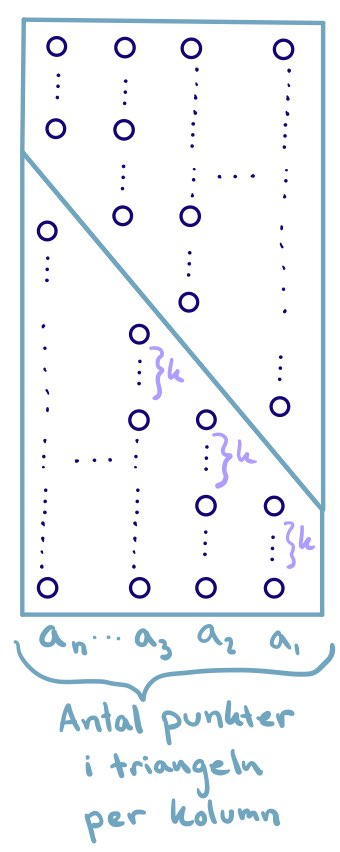
\includegraphics[width=0.5\textwidth]{graphics/86C79F60-B920-4AA3-A6CB-DEA00A8C58A6.jpeg}
    \caption{Rutnät av punkter. Bevis för summan av aritmetriska tlföljder. }
  \end{figure}
  
  Rektangelns höjd är $a_{1}+a_{n}$ (summan av det första och sista talet i talföljden) och dess bas är n. Rektangeln kan med denna information beräknas att ha $n\times(a_{1}+a_{n})$ prickar. Parallelltrapetsen består av hälften så många prickar som rektangeln, dvs $\frac{n\times(a_{1}+a_{n})}{2}$ prickar. Summan av en aritmetisk talföljd är alltså $\frac{n\times(a_{1}+a_{n})}{2}$.  
  
\end{example}

\begin{example}
  Vad är summan av de första $n$ udda talen, det vill säga $\sum_{k=1}^n 2k-1$?
  
  Svaret på frågan finner vi men hjälp av följande figur, som likt exemplet innan består av ett kvadratiskt rutnät av prickar. 
  
  \begin{figure}[h]
    \centering
    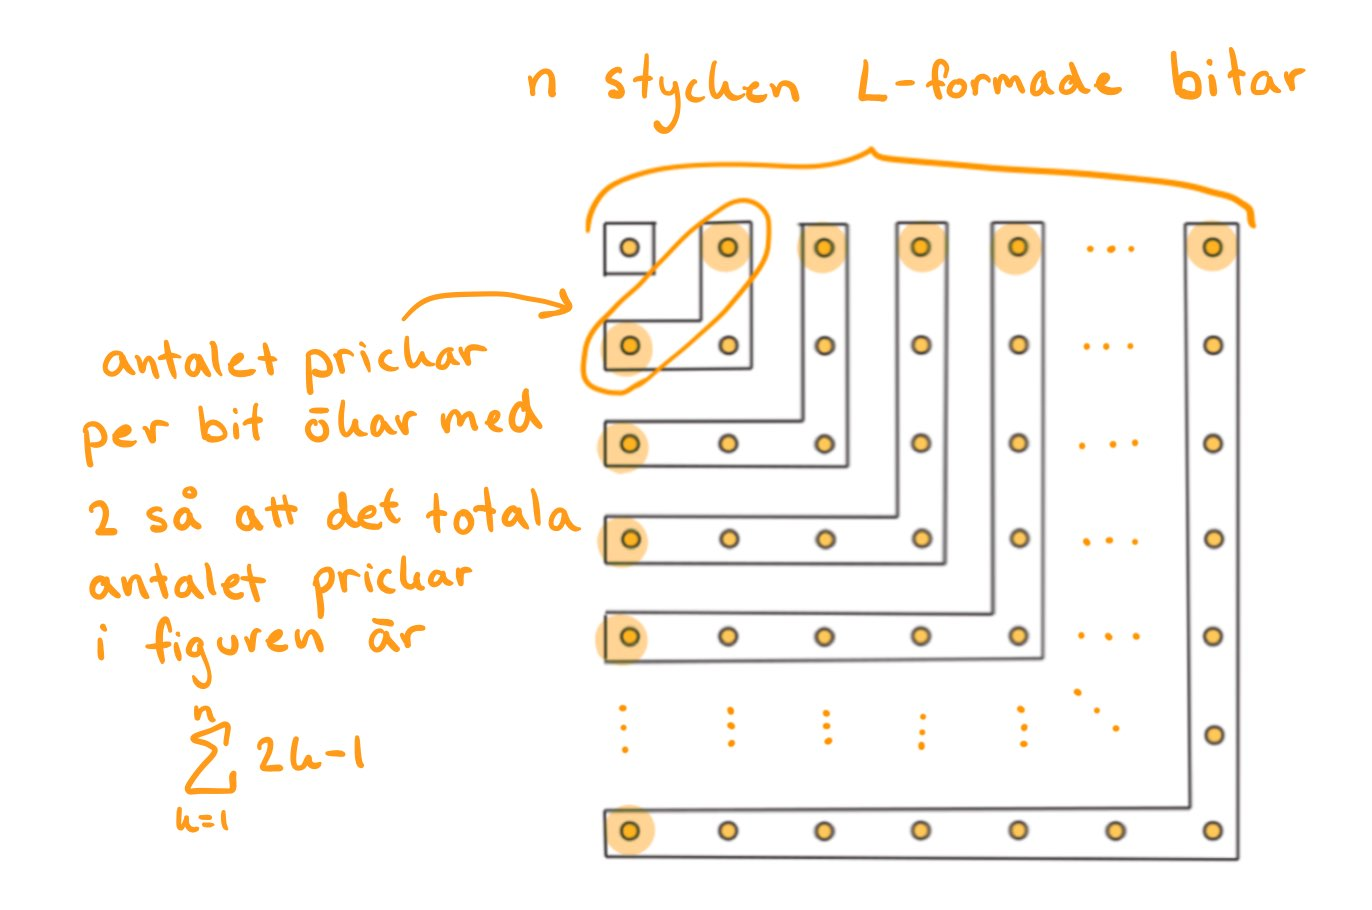
\includegraphics[width=0.5\textwidth]{graphics/Gauss square proof.jpg}
    \caption{Ett rutnät av $n\timesn$ punkter. Bevis att summan av de första $n$ udda talen är $n^2$.}
  \end{figure}
  
  Det totala antalet prickar i figuren är alltså $\sum_{k=1}^n 2k-1$ enligt resonnemanget i bilden ovan. Eftersom figuren är kvadratisk så kan vi även räkna antalet prickar i figuren genom att multiplicera sidorna $n\times n=n^2$. Svaret på frågan är därför $n^2$. 
\end{example}

\begin{example}\label{example_counting_all_subsets}
  Bevisa att $\sum_{k=0}^n \binom{n}{k} = 2^n$.

  \begin{proof}
    Vi bevisar detta genom att visa att både vänster och höger led räknar antalet delmängder till en mängd av $n$ element, oavsett delmängdernas storlek.\sidenote[][]{Man kan också betrakta detta som att vi räknar antalet binära strängar av längd $n$ på två sätt, eftersom det finns en enkel bijektion mellan sådana och delmängder till en mängd $X$ av storlek $n$.
    
    Specifikt så fixerar vi en numrering av elementen av $X$, och säger att givet en binär sträng $x_1x_2\ldots x_n$ så får vi en delmängd $A\subseteq X$ genom att det första elementet av $X$ ligger i $A$ om $x_1=1$, det andra om $x_2=2$, och så vidare. På motsvarande sätt kan vi konstruera en binär sträng givet en delmängd.}

    För vänster led kan vi observera att antalet delmängder oavsett storlek är summan av antalet delmängder av varje given storlek. Vi vet sedan innan att en delmängd av storlek $k$ av en mängd av storlek $n$ kallas en kombination, och det finns $\binom{n}{k}$ stycken sådana. Alltså är det totala antalet delmängder $\sum_{k=0}^n \binom{n}{k}$, som önskat.

    För höger led använder vi multiplikationsregeln. För varje element i vår mängd har vi två val -- antingen tar vi med elementet, eller inte -- och vi har totalt $n$ stycken element för vilka vi behöver göra detta val. Så om vi multiplicerar antalet val vi har varje gång får vi $2\cdot2\cdot\ldots\cdot2 = 2^n$ stycken delmängder, som önskat.
  \end{proof}
\end{example}

\begin{proposition}[Pascals Identitet]
  För $1 \leq k \leq n$ gäller det att\sidenote[][]{Den här likheten säger exakt att Pascals triangel faktiskt innehåller binomialkoefficienterna.}
  
  \begin{marginfigure}
    \includegraphics{graphics/pascals_triangle.png}
  \end{marginfigure}
  $$\binom{n}{k} = \binom{n-1}{k-1} + \binom{n-1}{k}.$$

  \begin{proof}[Algebraiskt bevis]
    \begin{align*}
      \binom{n-1}{k-1} + \binom{n-1}{k} &= \frac{(n-1)!}{(k-1)!((n-1)-(k-1))!} + \frac{(n-1)!}{k!((n-1)-k)!}\\
      &= (n-1)!\left(\frac{k}{k!(n-k)!} + \frac{(n-k)}{k!(n-k)!}\right)\\
      &= (n-1)!\frac{k + (n - k)}{k!(n-k)!}\\
      &= \frac{n!}{k!(n-k)!} = \binom{n}{k}.
    \end{align*}    
  \end{proof}

  \begin{proof}[Kombinatoriskt bevis]
    Låt $X$ vara en mängd av storlek $n$. Vi vet att $\binom{n}{k}$ räknar antalet delmängder av storlek $k$ till $X$. Låt oss komma på ett annat sätt att räkna antalet delmängder av storlek $k$, och se att det ger oss höger led.
    Välj ett godtyckligt element $x \in X$. Vi låter V beteckna alla delmängder till X som innehåller $x$, dvs $V=\{A\subseteq X:x\in A\} =\{ \{ x\} \cup B | B \subseteq X \backslash \{ x\} , |B|=k-1\}$, och vi låter H beteckna alla delmängder till X som inte innehåller x, dvs $H=\{A\subseteq X:x\notin A\} =\{A \subseteq X \backslash \{ x\} , |A|=k\}$. Vi ser att V och H är disjunkta och att unionen av dem är potensmängden av X. Idén är att räkna antalet delmängder av storlek k som tillhör V och H, och sedan använda additionsregeln för att räkna antalet delmängder av storlek k till X. 
    V innehåller redan elementet x vilket gör att vi har n-1 element kvar att välja från och k-1 val kvar att göra. Antalet element av storlek k i V är därför $\binom{n-1}{k-1}$.
    H innehåller inte elementet x vilket gör att vi har n-1 element att välja från och väljer ut k element. Antalet element av storlek k i H är alltså $\binom{n-1}{k}$. Notera att om n=k så är $\binom{n-1}{k}=0$ eftersom vi inte kan välja ut k element från k-1 element. 
    Till sist använder vi additionsregeln och får att antalet delmängder av storlek k till X är $\binom{n-1}{k-1} +\binom{n-1}{k}$. Så $\binom{n}{k}=\binom{n-1}{k-1}+\binom{n-1}{k}$. 
  \end{proof}
\end{proposition}

\section{Binomialsatsen}

\begin{theorem}[Binomialsatsen]
  För varje heltal $n\geq 0$ gäller det att\sidenote[][]{Lägg märke till att vi inte är så precisa kring vad $x$ och $y$ är. I versionen ni lärde er i gymnasiet är de två reella tal, men egentligen är det här en likhet mellan polynom, som gäller mycket mer allmänt. Vi använder ju inte några specifika egenskaper hos de reella talen i det här beviset, bara räkneregler för polynom. När ni läser en kurs i algebra kommer ni se hur generellt den sortens räkningar fungerar.}
  $$(x + y)^n = \sum_{k=0}^n \binom{n}{k}x^{n-k}y^k$$
  \begin{proof}
    Studera uttrycket
    $$(x + y)^n = (x + y)(x + y)\ldots(x + y).$$

    Vad är det vi gör när vi expanderar ut detta uttrycket? Jo, vi väljer för varje parentes om vi tar ett $x$ eller ett $y$ -- eller uttryckt i kombinatoriska termer, vi bildar ett ord ur alfabetet $\{x, y\}$. Så för $n = 3$ får vi till exempel att
    $$(x+y)(x+y)(x+y) = xxx + xxy + xyy + yxx + yxy + yyy.$$

    Sedan kommer vi ihåg att multiplikation är kommutativt, så $xyy = yxy$. Alltså spelar det ingen roll i vilken ordning vi gjorde valen, bara hur många gånger vi valde $x$ och hur många gånger vi valde $y$.\sidenote[][]{Alltså, formulerat på ett annat sätt, etiketterna av ``när valdes vilken'' spelar ingen roll.}

    Så antalet gånger vi får en term som är lika med $x^{n-k}y^k$ kommer alltså vara antalet $\{x, y\}$-strängar med $k$ stycken $y$. Det antalet är så klart samma som antalet sätt att välja $k$ platser att skriva $y$ ur den totala mängden av $n$ platser -- det vill säga $\binom{n}{k}$.

    Vi har alltså sett att koefficienten framför $x^{n-k}y^k$ när vi förenklat uttrycket kommer att vara $\binom{n}{k}$. Eftersom detta argument fungerar för varje $k$ har vi bevisat satsen.
  \end{proof}
\end{theorem}

\begin{example}
  Ge ett algebraiskt och ett kombinatoriskt bevis för att
  $$3^n = \sum_{k=0}^n \binom{n}{k}2^k.$$

  \begin{proof}[Kombinatoriskt bevis]
    Låt oss räkna antalet ternära strängar\sidenote[][]{Det vill säga strängar med alfabetet $\{0,1,2\}$.} av längd $n$ på två olika sätt. Det enkla sättet är att använda multiplikationsprincipen -- för varje bokstav har vi tre val, och vi behöver välja $n$ gånger, alltså blir produkten av antalet val för varje gång $3^n$.

    Ett annat sätt att räkna detta är att dela upp efter hur många ettor ordet innehåller. Först väljer vi antalet ettor, sedan väljer vi var ettorna skall stå, och till sist väljer vi vad resten av bokstäverna skall vara för något.

    Givet att vi vet att vi skall ha $k$ stycken ettor, och vi vet var de skall stå, så har vi $n-k$ bokstäver kvar att göra ett val för -- och nu har vi bara två val, eftersom vi inte får välja ettor utan bara nollor och tvåor. Så enligt multiplikationsprincipen multiplicerar vi antalet val vi har i varje fall och får att det finns $2^{n-k}$ sätt att fylla i resten av ordet med nollor och tvåor.

    Givet att vi vet att vi skall ha $k$ stycken ettor, hur många olika strängar kan vi skapa? Antalet sätt att välja var ettorna skall stå är precis antalet kombinationer av $k$ element från mängden av platser, $[n]$, och vi vet att det är $\binom{n}{k}$. När vi väl valt var ettorna skall stå kan vi fylla i resten på $2^{n-k}$ sätt, som vi såg i föregående stycket, så multiplikationsprincipen ger oss att det måste finnas $\binom{n}{k}2^{n-k}$ strängar av längd $n$ med $k$ stycken ettor.

    Till slut vet vi att det totala antalet ternära strängar måste vara summan av detta över alla $k$, enligt additionsprincipen. Så om vi summerar detta får vi att det finns
    $$\sum_{k=0}^n \binom{n}{k}2^{n-k}$$
    ternära strängar. Efter att ha tillämpat likheten $\binom{n}{k} = \binom{n}{n-k}$ och vänt på indexeringen i summan ser vi att detta är precis höger led i ekvationen vi gav. (Alltså båda summor beskriver samma summa men vänt, så sista termen i andra summan är samma som första termen i första summan osv.)
        $$\sum_{k=0}^n \binom{n}{n-k}2^{n-k}=\binom{n}{n}2^n+\binom{n}{n-1}2^{n-1}+\cdots+\binom{n}{1}2^1+\binom{n}{0}2^0$$
    $$\sum_{k=0}^n \binom{n}{k}2^k=\binom{n}{0}2^0+\binom{n}{1}2^{1}+\cdots+\binom{n}{n-1}2^n-1+\binom{n}{n}2^n$$

    Så 
    $$\sum_{k=0}^n \binom{n}{n-k}2^{n-k}=\sum_{k=0}^n \binom{n}{k}2^k$$
  \end{proof}

  \begin{proof}[Algebraiskt bevis]
    Vi använder binomialsatsen och ser att
    \begin{align*}
      3^n &= (1+2)^n\\
      &= \sum_{k=0}^n \binom{n}{k}1^{n-k}2^k = \sum_{k=0}^n \binom{n}{k}2^k.
    \end{align*}
  \end{proof}
\end{example}

\section{Omordningar}

\begin{definition}
  En omordning\sidenote[][]{Engelska \emph{rearrangement}, det verkar inte finnas ett helt inarbetat svenskt ord för detta, så omordning får fungera, om än klumpigt.} av en $X$-sträng $s$ är en annan $X$-sträng $s'$ där varje element i $X$ förekommer lika många gånger i $s'$ som i $s$. Specifikt måste alltså $s$ och $s'$ vara av samma längd.
\end{definition}

\begin{example}
  Det finns sex omordningar av $ABBA$:
  $$ABBA, ABAB, AABB, BAAB, BABA, BBAA.$$
\end{example}

\begin{proposition}\label{proposition_count_binary_rearrangements}
  Om $s$ är en binär sträng av längd $n$ med $k$ stycken ettor finns det $\binom{n}{k}$ stycken omordningar av $s$.
  \begin{proof}
    Vi behöver helt enkelt räkna antalet binära strängar av längd $n$ som har $k$ stycken ettor. För att konstruera en sådan behöver vi helt enkelt välja på vilka platser det skall stå en etta -- alltså välja en delmängd av $k$ platser av de totalt $n$ platserna. Detta vet vi att vi kan göra på $\binom{n}{k}$ sätt.
  \end{proof}
\end{proposition}

\section{Kompositioner}

Antag att vi vill fördela ut $n$ stycken osärskiljbara objekt bland $k$ särskiljbara människor.

\begin{example}
  Tre stycken lärare konkurrerar om två stycken äpplen de har fått av sina elever. På hur många olika sätt kan äpplena fördelas ut?

  Här är $n=3$ och $k=2$. Det finns sex olika sätt:
  \begin{table}[h]
    \begin{tabularx}{0.7\textwidth}{ccc}
    Äpplen för A & Äpplen för B      & Äpplen för C \\ 
    \midrule
    2 & 0 & 0\\
    1 & 1 & 0\\
    1 & 0 & 1\\
    0 & 2 & 0\\
    0 & 1 & 1\\
    0 & 0 & 2
    \end{tabularx}
    \end{table}
\end{example}

\begin{proposition}\label{proposition_indist_objs_dist_persons}
  Det finns $\binom{n+k-1}{k-1} = \binom{n+k-1}{n}$ sätt att fördela $n$ osärskiljbara föremål mellan $k$ särskiljbara personer.

  \begin{proof}
    Metoden för det här beviset brukar kallas för ett pinnar-och-stjärnor-argument.\sidenote[][]{Engelska \emph{stars and bars argument}.}

    Vi studerar ord ur alfabetet $\{*,|\}$ med $k-1$ stycken pinnar och $n$ stycken stjärnor. Till exempel om $n=6$ och $k=5$
    $$**||*|*|**$$

    Vi tolkar detta ordet som en fördelning av föremål till personer såsom följer: Person ett får alla  stjärnor innan första strecket, person två alla mellan första och andra strecket, och så vidare, tills person $k$ får alla stjärnor efter det sista strecket. I vårt exempel får alltså person ett två föremål, person två inga, person tre och fyra ett var, och person fem får två.

    Detta etablerar en bijektion mellan våra ord och fördelningarna till personer. Vi vet från Proposition \ref{proposition_count_binary_rearrangements}\sidenote[][]{Den propositionen handlar om binära strängar, men vi har alfabetet $\{*,|\}$ -- det spelar så klart ingen roll för antalet vad vi kallar våra bokstäver.} hur man räknar antalet sådana ord -- våra ord har längd $n + k -1$ (de innehåller $n$ stjärnor och $k-1$ streck) och $k-1$ av dem är av ena typen, så det måste finnas totalt $\binom{n + k - 1}{k - 1}$ ord, och alltså lika många fördelningar.
  \end{proof}
\end{proposition}

\begin{example}
  Hur många lösningar har ekvationen $x + y + z = 15$, ifall vi kräver att $x$, $y$, och $z$ alla skall vara positiva heltal?

  Vi kan se det här som en variant av problemet med att fördela osärskiljbara objekt mellan särskiljbara personer, där objekten är ettor och personerna är våra tre variabler. 
  
  Vi börjar med att ge varje variabel en etta, eftersom alla måste vara större än noll. Sedan har vi tolv ettor kvar att fördela mellan tre variabler, så Proposition \ref{proposition_indist_objs_dist_persons} säger oss att det finns $\binom{12 + 3 -1}{3 - 1} = \binom{14}{2} = 91$ lösningar.
\end{example}

\begin{definition}
  I allmänhet är antalet sätt att skriva $n$ som en summa av ett godtyckligt antal positiva heltal, där ordningen vi skrivar summan i spelar roll\sidenote[][]{$1+4$ och $4+1$ är alltså olika kompositioner av $5$.}, antalet \emph{kompositioner}\sidenote[][]{Inte att blanda ihop med \emph{kombinationer}, trots ordens snarlikhet.} av $n$. Vi studerade alltså just antalet kompositioner av längd $3$ av $15$.
\end{definition}

\section{Multinomialkoefficienter}

\begin{example}
  Hur många omordningar finns det av ordet $SPAPASTA$?\sidenote[][]{Ursprungligen ville jag ha det rimligare ordet \emph{pastasås}, men \LaTeX\ gillar visst inte \emph{Å} i ekvationer.}

  Det har $2$ stycken $S$ och $P$, $3$ stycken $A$, och ett $T$. Vi kan skapa en omordning av detta ordet genom att först välja var vi placerar $A$na -- det kan vi göra på $\binom{8}{3}$ sätt, eftersom vi har åtta platser och tre $A$n. När vi placerat ut dem har vi $8 - 3 = 5$ sätt att placera ut våra två $S$, så vi har $\binom{5}{2}$ val för hur vi gör det.

  Likaledes har vi $\binom{3}{2}$ sätt att placera ut våra $P$n, och till slut $\binom{1}{1}$ enda sätt att placera ut vårt $T$. Sammantaget blir det alltså
  \begin{align*}
    \binom{8}{3}\binom{5}{2}\binom{3}{2}\binom{1}{1} &= \frac{8!}{3!5!}\frac{5!}{2!3!}\frac{3!}{2!1!}\frac{1!}{1!0!}\\
    &= \frac{8!}{3!2!2!1!}
  \end{align*}
\end{example}

\begin{definition}
  För varje heltal $n$ och varje samling av heltal $k_1, k_2, \ldots, k_r$ sådana att $k_1 + k_2 + \ldots + k_r = n$ betecknar vi \emph{multinomialkoefficienten} med
  $$\binom{n}{k_1, k_2, \ldots, k_r} = \frac{n!}{k_1!k_2!\ldots k_r!}.$$

  Notera att våra vanliga binomialkoefficienter är specialfallet när $r=2$,
  $$\binom{n}{k} = \binom{n}{k, n-k} = \binom{n}{n-k}.$$
\end{definition}

\begin{proposition}
  Antag att $s$ är en $X$-sträng av längd $n$, som innehåller $k_1$ stycken $x_1$, $k_2$ stycken $x_2$, och så vidare, upp till $k_r$ stycken $x_r$ -- så $k_1 + k_2 + \ldots k_r = n$. Antalet omordningar av $s$ ges av multinomialkoefficienten $\binom{n}{k_1, k_2, \ldots, k_r}$.

  \begin{proof}
    Låt $R$ vara antalet omordningar av $s$. Vi använder återigen ``räkna samma sak på två olika sätt''-metoden. Den här gången är vad vi vill räkna antalet permutationer av längd $n$ ur alfabetet\sidenote[][]{Så i fallet där vårt ord är $SPAPASTA$ blir $$X' = \{S^1, S^2, P^1, P^2, A^1, A^2, A^3, T^1\}.$$
    
    Vi tar helt enkelt varje bokstav och ger den en etikett, så att bokstäverna blir särskiljbara.}
    \begin{align*}
      X' = \{&x_1^1, x_1^2, \ldots, x_1^{k_1},\\
             &x_2^1, x_2^2, \ldots, x_2^{k_2},\\
             &\qquad\vdots\\
             &x_r^1, x_r^2, \ldots, x_r^{k_3}\}.
    \end{align*}

    Eftersom $X'$ har exakt $n$ bokstäver vet vi att antalet permutationer av det alfabetet är precis $n!$.

    Låt oss nu räkna på ett mer komplicerat sätt. Vi kan också skapa oss en permutation av $X'$ genom att först välja en omordning av $s$, och sedan välja ett sätt att sätta etiketter på bokstäverna i den omordningen.\sidenote[][]{Så vi väljer en omordning av $SPAPASTA$, till exempel $ASPTAPAS$, och sätter sedan etiketter på bokstäverna för att få till exempel $A^2S^1P^2T^1A^1P^1A^3S^2$, vilket är en permutation av $X'$.}

    Om vi bara studerar våra $x_1$ i omordningen av $s$ så har vi $k_1$ stycken, och vi skall sätta etiketter mellan $1$ och $k_1$ på dem. Det kan vi göra på $k_1!$ sätt. Det samma gäller för varje annan bokstav, så multiplikationsprincipen säger oss att det totala antalet sätt att sätta etiketter måste vara $k_1!k_2!\ldots k_r!$. Det totala antalet permutationer av $X'$ måste alltså vara $R$, antalet omordningar, gånger detta, så vi har sett att 
    $$n! = Rk_1!k_2!\ldots k_r!$$
    och om vi löser detta för $R$ får vi precis den sökta satsen.
  \end{proof}
\end{proposition}

\begin{theorem}[Multinomialsatsen]
  Det gäller att
  $$(x_1 + x_2 + \ldots + x_r)^n = \sum_{\substack{k_1, k_2, \ldots, k_r \geq 0\\k_1 + k_2 + \ldots + k_r = n}} \binom{n}{k_1, k_2, \ldots, k_r} x_1^{k_1} x_2^{k_2} \ldots x_r^{k_r}$$

  \begin{proof}
    Precis samma argument som för binomialsatsen fungerar här.
  \end{proof}
\end{theorem}

\section{Övningar}

\begin{xca}
  I Exempel \ref{example_triangular_numbers} såg vi att
  $$\sum_{k=1}^n k = \frac{n(n+1)}{2}$$
  genom att studera en kvadrat av $(n+1)\times(n+1)$ punkter, och observera att den sökta summan räknar antalet punkter under diagonalen i figuren. Sedan använde vi ett algebraiskt argument för att få en formel för detta antal.

  En uppmärksam läsare kanske lägger märke till att $\frac{n(n+1)}{2} = \binom{n+1}{2}$, vilket ju också räknar antalet kombinationer av två element ur en mängd av $n+1$ element. Kan du komma på ett \emph{kombinatoriskt} bevis för varför antalet element under diagonalen på kvadraten är samma sak som antalet kombinationer av $2$ element från en mängd av $n+1$ element?
\end{xca}

\begin{xca}
  I en sidnot till Exempel \ref{example_counting_all_subsets} nämnde vi att det också går att se problemet som att räkna binära strängar av längd $n$, via en bijektion mellan sådana och delmängder till en mängd.

  Kan du skriva ett kombinatoriskt bevis för att $\sum_{k=0}^n \binom{n}{k} = 2^n$ som resonerar om binära strängar istället för om delmängder till en mängd?
\end{xca}

\begin{xca}
  Hur många heltalslösningar finns det till $x + y + z = 43$, om vi kräver att $x \geq 1$, $y \geq 17$, och $z \geq 5$?
\end{xca}

\begin{xca}
  Hur många omordningar finns det av ordet $54240244$?

  Hur många omordningar finns det av det ordet som inte börjar med en nolla?
\end{xca}

\begin{xca}
  Hur många ternära strängar av längd $2n$ finns det, där ettorna bara får dyka upp på udda positioner?
\end{xca}

\begin{xca}
  Låt $m$ och $w$ vara positiva heltal. Ge ett kombinatoriskt bevis för att det, för varje $0 \leq k \leq m + w$, gäller att
  $$\sum_{j=0}^k \binom{m}{j}\binom{w}{k-j} = \binom{m + w}{k}.$$
\end{xca}

\newpage
\section{Lösningsförslag}

\begin{xca}
\begin{proof}
  \begin{figure}[h]
    \centering
    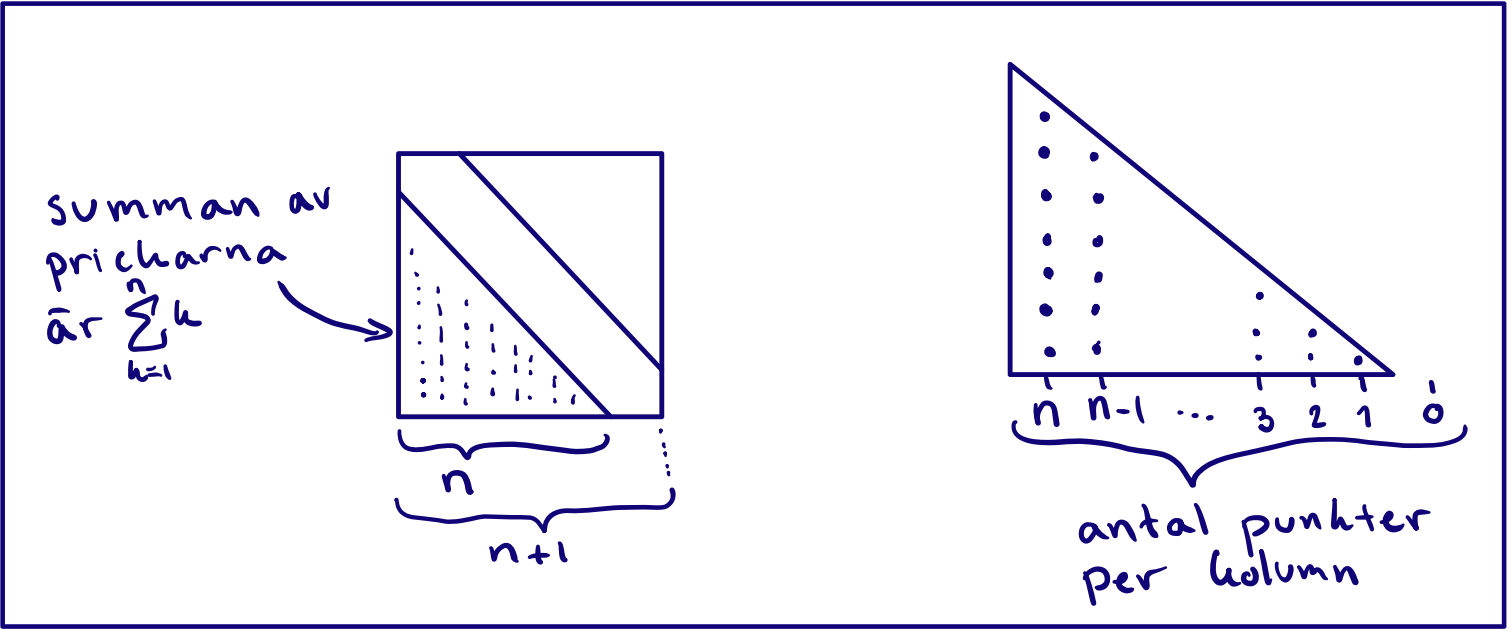
\includegraphics[]{graphics/Kombinatorik F 2 ls1.png}
  \end{figure}
$\binom{n+1}{2}$ är antalet sätt vi kan välja ut delmängder av storlek $2$ från $n+1$ element. Ett sätt att räkna detta är att välja ett godtyckligt element och kolla antalet sätt som detta element kan paras med resten av de kvarvarande $n$ stycken elementen. Detta blir $\binom{n}{1}=n$ sätt eftersom vi vill välja ut ett till element och vi har $n$ element att välja mellan.\\
Nästa steg är att välja ett nytt godtyckligt element och kolla antalet sätt osm detta element kan paras med resten av de $n-1$ kvarvarande elementen. Detta blir $\binom{n-1}{1}=n-1$ sätt.\\ Denna process upprepas tills alla element har valts och vi kan sedan använda additionsregels för att hitta totala antalet sätt att välja ut delmängder av storlek $2$ från $n+1$ element. \\
Vi kan uttrycka detta som $\binom{n}{1}+\binom{n-1}{1}+\cdots + \binom{2}{1}+\binom{1}{1}=n+(n-1)+\cdots +2+1=\sum_{k=1}^nk$\\
Exempel på hur processen tar formen av en triangel:
 \begin{figure}[h]
    \centering
    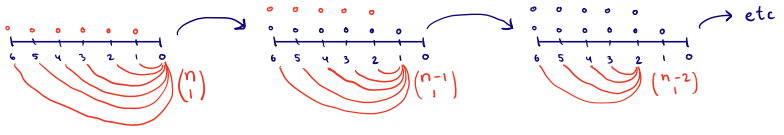
\includegraphics[width=0.5\textwidth]{graphics/kombinatorik ls1.png}
  \end{figure}
\end{proof}
\end{xca}


\begin{xca}
Låt $X$ vara en mängd där $|X|=n$. Numrera elementen i $X$ från $1$ till $n$.\\

Vi vill hitta en bijektion mellan antalet delmängder till $X$ och binära strängar av längd $n$.\\
$"\rightarrow": $ Varje delmängd $ a\subseteq X $ kan göras om till en binär sträng av längd $n$, dvs $x_1,x_2,\ldots , x_n$, genom att låta $x_i=$ \Big \{ ${1,\, om \, i\in x \atop 0, \, om\, i \notin x}$ \\
$"\leftarrow": $ Dessa binära strängar kan göras om till delmängder igen genom att låta det $i$:te elementet i $X$ tillhöra delmängden omm $x_i=1$. BInära strängarna kan alltså ses som en unik kod som anger vilka element som är med i delmängden.\\

Vi vet från fl 1 att antalet binära strängar med $n$ element är $2^n$.\\
Från bijektionen vet vi att: $$\sum_{k=0}^n\binom{n}{k}=|\{A:A\subseteq X\}|=|\{\text{binära strängar av längd n}\}|=2^n$$
\end{xca}


\begin{xca}
För att lösa uppgiften kan vi andvända oss av kompositioner. Vi kan se problemet som att vi ska dela ut 43 "objekt" mellan 3 "personer". Vi börjar att ge alla "personer" tillräckligt med "objekt" för att villkoren ska uppfyllas. I vårat fall har vi att x får 1 objekt, y får 17 objekt och z får 5 objekt. Det betyder att vi har totalt $43-(1+17+5)= 20$ "objekt" kvar att dela ut på 3 personer. Vi löser detta med hjälp av proposition 11 (Det finns $\binom{n+k-1}{k-1}=\binom{n+k-1}{n}$ olika sätt att födela n osärskiljbara föremål mellan k särskiljbara personer). Notera att i propositionen finns det 2 olika sätt att lösa detta men det blir samma lösning på slutet så det spelar ingen roll vilken man väljer att räkna med.
$$\binom{n+k-1}{k-1}=\binom{n+k-1}{n}$$ där n är antalet objekt och k antalet personer.
$$\binom{n+k-1}{k-1}=\binom{20+3-1}{3-1}= \binom{22}{2}=\frac{22!}{2!20!}=231$$
Och med det andra sättet:
$$\binom{n+k-1}{n}=\binom{20+3-1}{20}= \binom{22}{20}=\frac{22!}{20!2!}=231$$
Alltså kan vi lösa problemet på 231 olika sätt.
\end{xca}

\begin{xca}
a) Ordet $54240244$ har:
\begin{itemize}
  \item 1 "5"
  \item 4 "4"
  \item 2 "2"
  \item 1 "0"
\end{itemize}
Eftersom vi har flest $4$or så väljer jag att först placera ut dem (spelar ingen roll vilken man börjar med). Vi har totalt 8 platser och 4 st $4$ vilket ger oss $\binom{8}{4}$ olika sätt att placera ut $4$orna.\\
Därefter vill vi placera ut nästa siffra. Låt oss fortsätta med $2$orna. Om vi vid varje omordning placerar ut $4$orna först koer det alltid finnas 4 tomma platser kvar för resterande siffror oavsett vart $4$orna placerades. (vi vet inte vart dem placerades bara att 4 platser ockuperats vilket ger oss $8-4=4$ platser kvar.) Därför har vi $\binom{4}{2}$ stycken val för $2$orna.\\
Vi fortsätter med $5$orna. Med samma princip som innan har vi nu $8-4-2=2$ platser kvar alltså har vi $\binom{2}{1}$ olika sätt att placera ut $5$.\\
Sist är $0$an och nu har vi bara 1 plats kvar så det ger oss $\binom{1}{1}$ olika sätt att placera ut $0$an. Detta kommer då ge oss:
$$\binom{8}{4}\binom{4}{2}\binom{2}{1}\binom{1}{1}=\frac{8!}{4!4!}\frac{4!}{2!2!}\frac{2!}{1!1!}\frac{1!}{1!0!}$$
$$=840$$
Svar: Det finns 840 olika omordningar.\\
b) Nu vill vi inte att $0$ ska vara först så vi börjar med att placera ut $0$. $0$ har då 7 platser att välja mellan, alla utom den första platsen. Vi får då $\binom{7}{1}$ lika val att placera ut $0$ (då vi har 1 $0$).\\
Vi fortsätteer med nästa siffra, ex $4$. Dem har då också 7 platser kvar ($7-1=6$ platser efter vi valt plats för $0$ men sen nu kan vi räkna med första platsen för $4$ får vara på plats 1. Skulle vi ha haft fler $0$or så kan vi bara subtrahera dem från antalet platser) Vi har  då $\binom{7}{4}$ olika sätt att placera ut $4$orna.\\
Resten har samma princip som innan. $2$orna har 3 platser kvar så $\binom{3}{2}$ olika sätt att placera ut dem, och sist $\binom{1}{1}$ olika sätt för $5$an.\\
Därför har vi:
$$\binom{7}{1}\binom{7}{4}\binom{3}{2}\binom{1}{1}=\frac{7!}{1!6!}\frac{7!}{4!3!}\frac{3!}{2!1!}\frac{1!}{1!0!}$$
$$=735$$
Vilket låter logiskt eftersom 735 är 7 åttondelar av 840 och det borde finnas lika många omordningar för varje plats 0 kan befinna sig på, så om vi tar bort en plats borde det vara samma som att ta bort en åttondel.
\end{xca}


\begin{xca}
Ternära strängar består av alfabetet $\{ 0, 1, 2\}$ så $X=\{ 0, 1, 2\}$

\begin{column}
\begin{tabular}{|c|c|c|c|c|c|c|c|c|c|c|}
\hline
Position i & $1$ & $2$ & $3$ & $\cdots$ & $n$ & $n+1$ & $n+2$ & $n+3$ & $\cdots$ & $2n$ $ \\
\hline
Element x_i & x_1 & x_2 & x_3 &$\cdots$ & x_n & x_{n+1} & x_{n+2} & x_{n+3} & $\cdots $ & x_{2n} \\
\hline
\end{tabular}
\end{column}
Där $x_i=$\Bigg \{ ${0\, eller\, 2 \, om\, i\, \ddot{a}r\, j\ddot{a}mn \atop 0,\, 1,\, eller\, 2\, om\, i\, \ddot{a}r\, udda}$

Det finns $n$ stycken udda positioner. Varje udda position har 3 val (0, 1, eller 2).\\
Det finns $n$ stycken jämna positioner. Varje jämn position har 2 val (0 eller 2)\\
Det finns därför totalt $3^n\times 2^n$ sätt att välja ternära strängar enligt multiplikationsprincipen från föreläsning 1.\\
Svar: $3^n\times 2^n$

\end{xca}

\begin{xca}
\begin{proof}
Låt A och B vara disjunkta mmängder där $|A|=m$ och $|B|=w$. Höger led är då antalet delmängder av storlek $k$ till $X=A\cup B$. Vi vill visa att vänster led räknar samma sak.\\
Delmängder till $X$ av storlek $k$ kommer innehålla element från $A$ och/eller från $B$. Säg att en delmängd innehåller $j$ element från $A$, då måste resten av elementen komma från $B$, dvs $k-j$ element.\\
Multiplikationsprincipen säger att antalet sätt att välja $j$ element från $A$ (dvs\,$\binom{m}{j}$) multiplicerat med antalet sätt att välja $k-j$ element från $B$ (dvs\, $\binom{w}{k-j}$) är lika med antalet sätt vi kan välja $j$ element från $A$ och $k-j$ element från $B$ (dvs\, $\binom{m}{j} \binom{w}{k-j}$).\\
Detta gäller för då $j\in \{0,1, \ldots , k \}$, vilket täcker alla sätt att välja ett visst antal element från $A$. \\
Additionsprincipen säger att summan av alla dessa fall, $\sum_{j=0}^k \binom{m}{j} \binom{w}{k-j}$, också är antalet delmängder av storlek k.
\end{proof}
\end{xca}


%\bibliography{references}
%\bibliographystyle{plainnat}

\end{document}
